\documentclass[12pt]{article}
\usepackage[left=1.15in, right=1.15in, top=1in, bottom=1.5in]{geometry}
\usepackage{natbib}
\usepackage{verbatim}
\usepackage{setspace}
\usepackage{booktabs}
\usepackage{caption}
\usepackage{graphicx}
\usepackage{subcaption}
\usepackage{algorithm}
\usepackage{amsmath}
\usepackage{algpseudocode}
\usepackage{url}
\bibpunct[: ]{(}{)}{;}{a}{}{,} 
\usepackage{authblk}
\renewcommand\Authfont{\normalsize}
\renewcommand\Affilfont{\footnotesize}

\begin{document}
\title{A Generalized Approach to Combining Similarity and Eigenvector Analysis of Networks\thanks{Reserved for acknowledgments}}
\author[1]{Omar Lizardo\thanks{olizardo@soc.ucla.edu}}
\affil[1]{Department of Sociology, UCLA}

\renewcommand\Authands{ and }

\date{\normalsize \today}	
\maketitle

\newpage
\begin{abstract}
This paper presents a generalized approach to combining two key ideas in social network analysis: pairwise node similarity (based on local neighborhoods) and spectral ranking using feedback centralities (such as Bonacich's eigenvector scores). Building on the work of Alvarez-Socorro et al. (2015), who proposed weighing network edges by the dissimilarity between connected nodes to favor brokerage (connecting to well-connected, dissimilar others), the proposed generalization allows analysts to specify either dissimilarity or similarity as the preferred criterion. Weighing by similarity is argued to be more consistent with the idea of prominence as membership in a centralized core of well-connected nodes (closure). The generalized approach introduces parameters ($\alpha$ and $\beta$) to combine these two strategies, yielding a compromise ranking that accounts for both brokerage and closure. An analysis of the classic Florentine Families network demonstrates that the Medici family specializes in brokerage, ranking highest when a dissimilarity weight is used. In contrast, the Peruzzi family emerges as the most central when an approach that rewards similarity/closure is used.
\end{abstract}

\newpage
\section*{Introduction}
The standard approach to computing ``feedback'' based indices of node position in networks is due to the classic work of \citep{bonacich1972factoring-03e}. Here, the idea of feedback reduces to the more specific notion that a node's ranking in the resulting index---which can be interpreted as a ``centrality'' measure \citep{borgatti2006graph-theoretic-1a0}---is higher if it is connected to others who are themselves well connected. Thus, if the (undirected) adjacency relations in the network are represented in the (symmetric) matrix $\mathbf{A}$ with $a_{ij} = 1$ if nodes $i$ and $j$ are connected in the underlying graph, then the vector of standard Bonacich scores $\mathbf{s}$ can be obtained via the solution to the linear system:

\begin{equation}
    \lambda_{1}\mathbf{s} = \mathbf{A}\mathbf{s}
    \label{eq:bon}
\end{equation}

Where $\lambda_{1}$ is the leading (largest) eigenvalue of the adjacency matrix, also referred to as $\rho(\mathbf{A})$, or the ``spectral radius'' of the adjacency matrix. If $\lambda_{1}$ exists, then its associated $\mathbf{s}$ eigenvector also exists, and it is guaranteed (via the famous Perron-Frobenius theorem) to be composed of real non-negative scores, which can be used to induce a ranking on the nodes of the network \citep{vigna2016spectral-19a}.

\section*{Combining Similarity and Eigenvector Ranking}

In a recent contribution, \citet{alvarez-socorro2015eigencentrality-66c} propose to merge the Bonacich approach to feedback centrality scoring with the analysis of vertex similarity in networks \citep{leicht2006vertex-6f1}. Their basic idea is simple, proposing that we substitute the adjacency matrix in Equation~\ref{eq:bon} with a different matrix $\mathbf{W}$ which is defined as:

\begin{equation}
    \mathbf{W} = \mathbf{A} \odot (1 - \mathbf{S})
    \label{eq:ac1}
\end{equation}

Where $\mathbf{S}$ is a matrix of (local) vertex \textit{similarities} (making $1-\mathbf{S}$ a dissimilarity or distance matrix), and the $\odot$ operation refers to the element-wise ``dot'' product. In essence, what \citet{alvarez-socorro2015eigencentrality-66c} are doing is attaching the local vertex \textit{dissimilarity} score---bound to fall in the zero to one interval---as a \textit{weight} on each edge in the network, and then computing the standard Bonacich scores from the dissimilarity weighted adjacency matrix to rank nodes in the network. Note that this approach sets the dissimilarity scores of non-adjacent nodes to zero, making the results different from the spectral decomposition of the raw distance matrix $1 - \mathbf{S}$. 

This leads to the modified linear system:

\begin{equation}
    \lambda_1\mathbf{s} = \mathbf{W}\mathbf{s}
    \label{eq:ac2}
\end{equation}

There are many options from which to construct $\mathbf{S}$, but an attractive one is the Jaccard similarity $s^J$, because its complement $1-s^J$ returns a true metric distance (respecting the triangle inequality). In terms of the adjacency matrix, we can define the Jaccard similarity matrix as:

\begin{equation}
    \mathbf{S} = \frac{\mathbf{P}}{\mathbf{P}+\mathbf{Q}+\mathbf{Q}^T}
\end{equation}

With:

\begin{subequations}
\begin{equation}
    \mathbf{P} = \mathbf{A}^2
\end{equation}
\begin{equation}
    \mathbf{Q} = \mathbf{A}(1-\mathbf{A})
\end{equation}
\end{subequations}

Conceptually, the approach of \citet{alvarez-socorro2015eigencentrality-66c} is motivated by the idea that being connected to well-connected others who are also \textit{dissimilar} from you (because they are not linked to your neighbors) should matter more in determining node ranking than being connected to well-connected others who are also connected to your neighbors. Thus, theoretically, this approach merges the ``feedback'' reasoning animating the Bonacich prestige ranking approach with the ``brokerage'' reasoning of Burt's \citeyearpar{burt1995structural-5e8} theory of structural holes. 

Algorithm~\ref{alg:ac} presents pseudocode for a simple algorithm that implements Alvarez-Socorro et al.'s eigenvector-based node-scoring approach.

\begin{algorithm}[ht!]
\caption{Alvarez-Socorro's et al.'s \citeyearpar{alvarez-socorro2015eigencentrality-66c} Dissimilarity Scoring}
\label{alg:ac}
\begin{algorithmic}[1]
\Require $\mathbf{A}$ \Comment{$n \times n$ symmetric adjacency matrix}
\State $\mathbf{P} \gets \mathbf{A}^2$ \Comment{Common neighbors matrix}
\State $\mathbf{Q} \gets \mathbf{A}(1-\mathbf{A})$ \Comment{Non-shared neighbors matrix}
\State $\mathbf{S} \gets \mathbf{P} \div \left(\mathbf{P}+\mathbf{Q}+\mathbf{Q}^T\right)$ \Comment{Jaccard similarity matrix}
\State $\mathbf{D} \gets 1-\mathbf{S}$ \Comment{Jaccard distance matrix}
\State $\mathbf{W} \gets \mathbf{A} \odot \mathbf{D}$ \Comment{element-wise product between $\mathbf{A}$ and $\mathbf{D}$}
\State Compute $\mathbf{s}$ using Equation~\ref{eq:ac2} \Comment{The right dominant eigenvector of $\mathbf{W}$}
\State \Return $\mathbf{s}$ \Comment{$n \times 1$ column vector of non-negative scores}
\end{algorithmic}
\end{algorithm}

\section*{A Generalized Approach}
The \citet{alvarez-socorro2015eigencentrality-66c} approach to eigenvector scoring assumes that we want to characterize nodes as most central when their connectivity strategy combines a logic of proximity to the well-connected with a logic of brokerage between disconnected others. However, in some applications, the most central nodes may be those that combine a logic of proximity to the most central with \textit{closure}, that is, connecting to others who are also linked to their neighbors. 

This is particularly the case in networks that feature a core-periphery or ``nested shell'' structure with a well-connected group of nodes that are also mutually connected at the center and another set of less well-connected nodes at the periphery \citep{borgatti2000models-3c1}---also referred to as the ``rich club'' phenomenon \citep{colizza2006detecting}. In this case, eigenvector scoring of the \textit{similarity}-weighted adjacency matrix $\mathbf{S}$ would make more sense and likely yield a substantively different ranking of the nodes. 

Given these competing analytic aims, it would seem appropriate to generalize Alvarez-Socorro et al.'s approach to give analysts the flexibility to specify either dissimilarity (brokerage) or similarity (closure) as the preferred criterion for eigenvector-based node ranking, or perhaps attempt to balance between the two. 

One option would be to modify Equation~\ref{eq:ac1} as follows:

\begin{equation}
    \mathbf{W} = \mathbf{A} \odot \left[\mathbf{S}^\alpha \odot (1 - \mathbf{S})^\beta\right]
    \label{eq:gen}
\end{equation}

With the restrictions that $0 \geq \alpha \leq 1$ and $0 \geq \beta \leq 1$ and $\alpha + \beta \leq 1$.

Note that when $\alpha = \beta = 0$ in Equation~\ref{eq:gen}, then  $\mathbf{W} = \mathbf{A}$ and we recover the standard Eigenvector scores given by Equation~\ref{eq:bon}. When $\alpha = 0$ and $\beta = 1$, then $\mathbf{W} = \mathbf{A} \odot (1 - \mathbf{S})$, which is the same as Equation~\ref{eq:ac1}, and when apply Equation~\ref{eq:ac2}, we recover the dissimilarity-weighted eigenvector scores of \citet{alvarez-socorro2015eigencentrality-66c}. When $\alpha = 1$ and $\beta = 0$, then $\mathbf{W} = \mathbf{A} \odot \mathbf{S}$, and when we apply Equation~\ref{eq:ac2}, we recover scores that weigh the ranking by the focal node's \textit{similarity} to well-connected (direct and indirect) neighbors. Finally, when $\alpha > 0$ \textit{and} $\beta > 0$ then $\mathbf{W}$ is given by Equation~\ref{eq:gen}, and when we apply Equation~\ref{eq:ac2}, we recover a compromise ranking that takes both brokerage and closure relative to well-connected direct and indirect neighbors into account. 

The pseudocode for a revised version of Algorithm~\ref{alg:ac} implementing this idea is shown as Algorithm~\ref{alg:ol}.

\begin{algorithm}[ht!]
\caption{Proposed Algorithm for Generalized Similarity Scoring}
\label{alg:ol}
\begin{algorithmic}[1]
\Require $\mathbf{A}, \alpha, \beta$ \Comment{$n \times n$ symmetric adjacency matrix and two scalar parameters}
\Ensure $0 \geq \alpha \leq 1$
\Ensure $0 \geq \alpha \leq 1$
\Ensure $\alpha + \beta \leq 1$
\State $\mathbf{P} \gets \mathbf{A}^2$ \Comment{Common neighbors matrix}
\State $\mathbf{Q} \gets \mathbf{A}(1-\mathbf{A})$ \Comment{Non-shared neighbors matrix}
\State $\mathbf{S} \gets  \mathbf{P} \div \left(\mathbf{P}+\mathbf{Q}+\mathbf{Q}^T\right)$ \Comment{Jaccard similarity matrix}
\State $\mathbf{D} \gets 1-\mathbf{S}$ \Comment{Jaccard distance matrix}
\State $\mathbf{Z} \gets \mathbf{S}^\alpha \odot \mathbf{D}^\beta$ \Comment{Element-wise product of $\mathbf{S}^\alpha$ and $\mathbf{D}^\beta$}
\State $\mathbf{W} \gets \mathbf{A} \odot \mathbf{Z}$ \Comment{element-wise product between $\mathbf{A}$ and $\mathbf{Z}$}
\State Compute $\mathbf{s}$ using Equation~\ref{eq:ac2} \Comment{The right dominant eigenvector of $\mathbf{W}$}
\State \Return $\mathbf{s}$ \Comment{$n \times 1$ column vector of non-negative scores}
\end{algorithmic}
\end{algorithm}

\section*{Data Example}
To get a sense of how the generalized eigenvector similarity approach works, I analyze the oft-considered Florentine Families network of \citet{padgett1993robust-4cc}---also analyzed, inter alia, by \citet{alvarez-socorro2015eigencentrality-66c}. I construct the network by merging the marriage and business ties and linking two families if they are connected by either or both types of ties.\footnote{Data were obtained from the \texttt{R} package \texttt{networkdata} \citep{schoch-network-data}.} The network can therefore be represented by an undirected graph and its associated symmetric adjacency matrix. 

A point and line plot of the Florentine Families network is shown in Figure~\ref{fig:main}, using the standard \texttt{igraph} layout algorithm to determine node position \citep{csardi06}. The network shows, as has been observed in myriad previous analyses of this network, the Medici at the center of a ``star'' subsection of the graph, connected to alters who are not mutually connected. We should expect, therefore, that they would fare well in a feedback central measure, such as that proposed by Alvarez-Socorro et al's \citeyearpar{alvarez-socorro2015eigencentrality-66c} in which being connected to well-connected but locally dissimilar partners counts for more (and they show that in their paper). 

\begin{figure}[ht!]
    \centering
    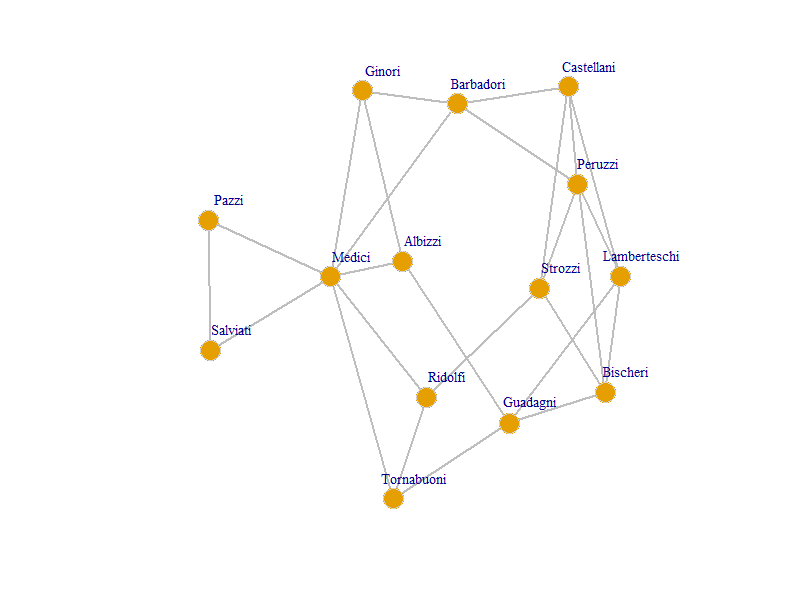
\includegraphics[width=0.8\linewidth]{medici.png}
    \caption{Combined Medici Marriage and Business Network}
    \label{fig:main}
\end{figure}

However, if we were thinking of centrality as being better indexed by being connected to well-connected others, who are themselves connected to your neighbors, then we should not expect the Medici to fare as well. Instead, it is the Peruzzi family, at the center of a ``wheel'' with connected spokes, who should be the most central. 

\begin{table}
\centering
\caption{Eigenvector-Based Scores for the Medici Network.}
\centering
\resizebox{\ifdim\width>\linewidth\linewidth\else\width\fi}{!}{
\begin{tabular}[t]{lclclclc}
\toprule
Node & Eig. & Node & Eig./Dis & Node & Eig./Sim & Node & Eig./Both\\
\midrule
Peruzzi & 1.000 & Medici & 1.000 & Peruzzi & 1.000 & Peruzzi & 1.000\\
Medici & 0.941 & Barbadori & 0.534 & Castellani & 0.754 & Lamberteschi & 0.786\\
Castellani & 0.794 & Guadagni & 0.405 & Lamberteschi & 0.682 & Bischeri & 0.765\\
Barbadori & 0.775 & Peruzzi & 0.389 & Bischeri & 0.655 & Castellani & 0.763\\
Lamberteschi & 0.754 & Tornabuoni & 0.385 & Strozzi & 0.518 & Strozzi & 0.644\\
Bischeri & 0.740 & Albizzi & 0.374 & Barbadori & 0.263 & Barbadori & 0.477\\
Strozzi & 0.722 & Ridolfi & 0.370 & Guadagni & 0.203 & Guadagni & 0.355\\
Guadagni & 0.555 & Strozzi & 0.344 & Ginori & 0.061 & Medici & 0.208\\
Ginori & 0.438 & Ginori & 0.326 & Medici & 0.045 & Ginori & 0.197\\
Ridolfi & 0.424 & Castellani & 0.309 & Albizzi & 0.018 & Albizzi & 0.092\\
Albizzi & 0.395 & Bischeri & 0.288 & Pazzi & 0.008 & Salviati & 0.062\\
Tornabuoni & 0.391 & Lamberteschi & 0.280 & Salviati & 0.008 & Pazzi & 0.062\\
Salviati & 0.100 & Pazzi & 0.044 & Ridolfi & 0.006 & Tornabuoni & 0.055\\
Pazzi & 0.100 & Salviati & 0.044 & Tornabuoni & 0.006 & Ridolfi & 0.055\\
Acciaiuoli & 0.000 & Acciaiuoli & 0.000 & Acciaiuoli & 0.000 & Acciaiuoli & 0.000\\
\bottomrule
\end{tabular}}
\end{table}


Table~\ref{tab:main} shows the results.\footnote{All scores are normalized to fall within the zero to one range.} The first two columns of the table show the rankings according to the standard \citet{bonacich1972factoring-03e} centrality and the \citet{alvarez-socorro2015eigencentrality-66c} scoring ($\alpha = 0$ and $\beta = 0$). We can see that both the Peruzzi and the Medici families emerge as most central when using the raw eigenvector scoring (with the Peruzzi slightly edging out the Medici for the top spot). However, we can see that once we adopt Alvarez-Socorro et al.'s approach ($\alpha = 0$ and $\beta = 1$), which rewards both well-connectedness \textit{and} brokerage, the Medici emerge as the undisputed most central actors in the network, consistent with Padgett and Ansell's \citeyearpar{padgett1993robust-4cc} classic analysis, which relied on the betweenness centrality (another metric that rewards brokerage). The Peruzzi, scored as the most central in the standard eigenvector scoring, drop to fourth place. 

The last two columns of the table show the rankings obtained from Equation~\ref{eq:gen}, first (columns five and six) using $\alpha = 1$ and $\beta = 0$ (giving all weight to being connected to well-connected others who are also adjacent to your other neighbors), and then using $\alpha = 0.15$ and $\beta = 0.85$ (columns seven and eight).\footnote{Informal experimentation suggested that selecting values for $\alpha$ and $\beta$ of similar magnitude resulted in ranks substantively indistinguishable from those in columns 5 and 6, indicating that the similarity dominates over the dissimilarity. Selecting parameters that favor dissimilarity weights yielded a ranking closer to a compromise.} 

From the similarity-based scoring, we can see that the Peruzzi are the undisputed most central actors in the network, while the Medici are fairly peripheral. The other top actors, according to this scoring, all belong to the well-connected core actors revolving around Peruzzi on the right-hand side of Figure~\ref{fig:main}. 

We can also see that the ``hybrid'' approach, as expected, produces a compromise ranking in which nodes that combine both brokerage and similarity-based connectivity strategies appear toward the top. The Barbadori family is notable in this respect: They are a distant second in the approach of \citet{alvarez-socorro2015eigencentrality-66c} and in sixth place when ranking nodes according to the similarity weight, but they appear in second place in the hybrid rank, suggesting they do a good job of combining both brokerage and closure connectivity strategies.  

\section*{Discussion and Concluding Remarks}
This short methodological note presents a generalized approach to combining the reasoning behind analyses of social networks that focus on pairwise similarities between nodes based on their local neighborhood \citep{leicht2006vertex-6f1} with spectral ranking based on the idea of feedback centralities, where nodes are central when they are directly and indirectly connected to central others \citep{bonacich1972factoring-03e}. Building on recent work by \citet{alvarez-socorro2015eigencentrality-66c} who propose to use the pairwise dissimilarities between nodes as a weight on each edge before estimating the usual Bonacich eigenvector rankings, I argue that in some settings it might be more desirable to weigh the edges by the \textit{similarity}, as this may be more consistent with the idea of prominence as membership in a centralized core of well-connected nodes. 

The generalized approach also allows us to \textit{combine} these two analytic strategies, ranking nodes highly when they hedge their bets and combine both connectivity strategies. Analysis of the classic Florentine Families dataset of \citet{padgett1993robust-4cc} reveals that, when considering two different connectivity strategies, the much heralded Medici family emerges as \textit{brokerage specialists}: Undisputedly the top nodes when the pairwise dissimilarities between connected dyads are used as edge weights before eigenvector ranking. When we use ranking approaches that reward belonging to well-connected cores, however, the Medici emerge as largely peripheral nodes in the network. 

The approach proposed here can also be extended to other families of feedback-based centralities. For instance, the famous all-paths centrality due to \citet{katz1953new-19a} could be extended in the same way, by substituting $\mathbf{W}$ for $\mathbf{A}$ in the usual calculation. Here, we would consider them central if they share many paths with many others, where the paths are weighted by either similarity or dissimilarity, depending on the application.  The same approach can be used with other attenuated path-based measures of node position, such as communicability centrality \citep{estrada2010network-294}, which can be fruitfully combined with similarity/dissimilarity analysis in the same way. 




\newpage
\bibliography{references}
\bibliographystyle{asr}

\end{document}
